\documentclass{article}
\usepackage[utf8]{inputenc}
\usepackage{graphicx}
\usepackage{listings}
\usepackage{xcolor}
\usepackage{fancyhdr}
\usepackage{hyperref}
\usepackage{geometry}

\geometry{margin=1in}

\lstset{
    backgroundcolor=\color{lightgray!30},
    basicstyle=\ttfamily\small,
    breaklines=true,
    captionpos=b,
    commentstyle=\color{green},
    frame=single,
    keywordstyle=\color{blue},
    showstringspaces=false,
    stringstyle=\color{purple},
}

\hypersetup{
    colorlinks=true,
    linkcolor=blue,
    filecolor=magenta,
    urlcolor=cyan,
}

\pagestyle{fancy}
\fancyhf{}
\rhead{Jupyter Notebook Report}
\lhead{Generated: \today}
\cfoot{\thepage}


\begin{document}

\begin{center}
\Large\textbf{Jupyter Notebook Assignment Report}

\vspace{0.5cm}
\normalsize
Student: Nishal Sukumar

Assignment: Nishal_Sukumar_Assignment_1

Date: 2025-04-11 19:35
\end{center}

\vspace{1cm}


\vspace{0.5cm}
\noindent\colorbox{lightgray}{\textbf{Cell 1 (code)}}
\vspace{0.3cm}


\begin{lstlisting}[language=Python]
\# Import libraries
import pandas as pd
import numpy as np
import seaborn as sns
import matplotlib.pyplot as plt
from sklearn.datasets import fetch\_california\_housing
from sklearn.model\_selection import train\_test\_split
from sklearn.linear\_model import LinearRegression
from sklearn.metrics import mean\_squared\_error, r2\_score
\end{lstlisting}


\vspace{0.5cm}
\noindent\colorbox{lightgray}{\textbf{Cell 2 (code)}}
\vspace{0.3cm}


\begin{lstlisting}[language=Python]
\# Load California housing dataset
california = fetch\_california\_housing()
df = pd.DataFrame(california.data, columns=california.feature\_names)
df['Target'] = california.target
\end{lstlisting}


\vspace{0.5cm}
\noindent\colorbox{lightgray}{\textbf{Cell 3 (markdown)}}
\vspace{0.3cm}


\begin{quote}
\textbackslash{}# ---- EDA ----
\end{quote}


\vspace{0.5cm}
\noindent\colorbox{lightgray}{\textbf{Cell 4 (code)}}
\vspace{0.3cm}


\begin{lstlisting}[language=Python]
\# Basic Info
print("Shape of dataset:", df.shape)
print("\\nFirst 5 rows:\\n", df.head())
print("\\nSummary statistics:\\n", df.describe())
\end{lstlisting}


\begin{verbatim}
stdout: Shape of dataset: (20640, 9)

First 5 rows:
    MedInc  HouseAge  AveRooms  AveBedrms  Population  AveOccup  Latitude  \
0  8.3252      41.0  6.984127   1.023810       322.0  2.555556     37.88   
1  8.3014      21.0  6.238137   0.971880      2401.0  2.109842     37.86   
2  7.2574      52.0  8.288136   1.073446       496.0  2.802260     37.85   
3  5.6431      52.0  5.817352   1.073059       558.0  2.547945     37.85   
4  3.8462      52.0  6.281853   1.081081       565.0  2.181467     37.85   

   Longitude  Target  
0    -122.23   4.526  
1    -122.22   3.585  
2    -122.24   3.521  
3    -122.25   3.413  
4    -122.25   3.422  

Summary statistics:
              MedInc      HouseAge      AveRooms     AveBedrms    Population  \
count  20640.000000  20640.000000  20640.000000  20640.000000  20640.000000   
mean       3.870671     28.639486      5.429000      1.096675   1425.476744   
std        1.899822     12.585558      2.474173      0.473911   1132.462122   
min        0.499900      1.000000      0.846154      0.333333      3.000000   
25%        2.563400     18.000000      4.440716      1.006079    787.000000   
50%        3.534800     29.000000      5.229129      1.048780   1166.000000   
75%        4.743250     37.000000      6.052381      1.099526   1725.000000   
max       15.000100     52.000000    141.909091     34.066667  35682.000000   

           AveOccup      Latitude     Longitude        Target  
count  20640.000000  20640.000000  20640.000000  20640.000000  
mean       3.070655     35.631861   -119.569704      2.068558  
std       10.386050      2.135952      2.003532      1.153956  
min        0.692308     32.540000   -124.350000      0.149990  
25%        2.429741     33.930000   -121.800000      1.196000  
50%        2.818116     34.260000   -118.490000      1.797000  
75%        3.282261     37.710000   -118.010000      2.647250  
max     1243.333333     41.950000   -114.310000      5.000010  

\end{verbatim}


\vspace{0.5cm}
\noindent\colorbox{lightgray}{\textbf{Cell 5 (code)}}
\vspace{0.3cm}


\begin{lstlisting}[language=Python]
\# Check for missing values
print("\\nMissing values:\\n", df.isnull().sum())
\end{lstlisting}


\begin{verbatim}
stdout: 
Missing values:
 MedInc        0
HouseAge      0
AveRooms      0
AveBedrms     0
Population    0
AveOccup      0
Latitude      0
Longitude     0
Target        0
dtype: int64

\end{verbatim}


\vspace{0.5cm}
\noindent\colorbox{lightgray}{\textbf{Cell 6 (code)}}
\vspace{0.3cm}


\begin{lstlisting}[language=Python]
\# Correlation heatmap
plt.figure(figsize=(10, 8))
sns.heatmap(df.corr(), annot=True, cmap='coolwarm', fmt=".2f")
plt.title("Correlation Heatmap")
plt.show()
\end{lstlisting}


\begin{verbatim}
<Figure size 1000x800 with 2 Axes>
\end{verbatim}


\begin{figure}[h]
\centering
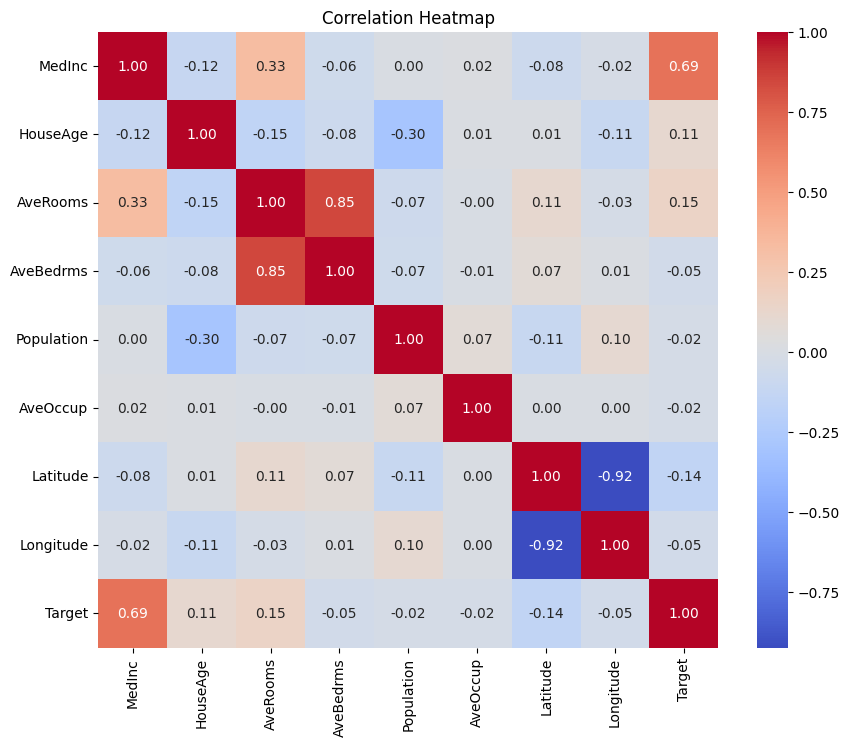
\includegraphics[width=0.8\textwidth]{images/image_1.png}
\caption{Output Image 1}
\end{figure}


\vspace{0.5cm}
\noindent\colorbox{lightgray}{\textbf{Cell 7 (code)}}
\vspace{0.3cm}


\begin{lstlisting}[language=Python]
\# Distribution of the target variable
sns.histplot(df['Target'], kde=True)
plt.title("Distribution of Target (Median House Value)")
plt.show()
\end{lstlisting}


\begin{verbatim}
<Figure size 640x480 with 1 Axes>
\end{verbatim}


\begin{figure}[h]
\centering
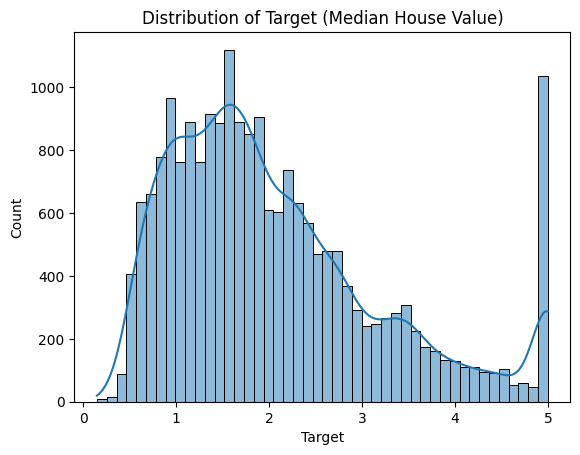
\includegraphics[width=0.8\textwidth]{images/image_2.png}
\caption{Output Image 2}
\end{figure}


\end{document}